\documentclass[a4paper,12pt]{article}
\usepackage[top=3cm, bottom=3cm, left=3cm, right=3cm]{geometry}	%dimension de la feuille
\usepackage[utf8]{inputenc}%codage linux
\usepackage[T1]{fontenc}%les fontes
\usepackage[french]{babel}%caractères français
\usepackage{amsmath}
\usepackage{amssymb}
\usepackage{mathrsfs}
\usepackage{hyperref}%liens pdf
\usepackage{listings}%pour mettre du code
\usepackage{color}%pour la couleur dans le code
\usepackage{graphicx}%pour \includegraphics
\usepackage{float}
\usepackage{longtable}
\usepackage[table]{xcolor}
\lstset{breaklines=true}
\usepackage{verbatim}
\usepackage{array}
\usepackage{svg}

%%%%%%%%%%%%%%%%%%%% Presentation %%%%%%%%%%%%%%%%%%%
\title{Informatique Répartie\\Rapport\\Sujet : Messagerie instantanée 2}
\author{Ingrid FIQUET\\Morgane LEGROS\\Florian MARTIN\\Thibault THÉOLOGIEN\\Youssef ZERHOUNI ABDOU}
\date{\today}


\begin{document}
	\begin{titlepage}
		\vfill
		\begin{figure}
			
\includegraphics[scale=0.3]{img/logoINSARouen.png}
		\end{figure}

		\maketitle

		\vfill
		\noindent \hrulefill

	\end{titlepage}


%%%%%%%%%%%%%%%%%%%% Corps %%%%%%%%%%%%%%%%%%%

\newpage
\tableofcontents{}

\newpage
\part{Introduction}
		\par Ce document concerne la réalisation d'une application de messagerie instantanée.
	\par Il s’agira d’une messagerie permettant à la fois le dialogue vers un utilisateur unique ou bien vers un ensemble d’utilisateurs.
	\par La discussion pourra être en audio conférence dans le cas d’un dialogue vers un unique utilisateur.
	\par Chaque utilisateur pourra dans les paramètres de son compte gérer la configuration du système de filtrage de la messagerie. \\

	\par En ce qui concerne les utilisateurs, la messagerie sera accessible par des utilisateurs humains ou bien par des utilisateurs virtuels.
	\par Les utilisateurs virtuels seront capables d’une discussion simple lors d’un dialogue avec un unique utilisateur.
	\par Enfin l’administrateur aura lui accès à l’ensemble des comptes utilisateurs et sera le seul autorisé à faire certaines actions telles que bannir un utilisateur par exemple. \\

	\par Cette messagerie instantanée sera supportée par tous les OS, accessible via tous les navigateurs et depuis tous types d’appareils (PC, smartphone).


\newpage
\part{Spécification}
	Les spécifications du projet ont été définies au début du projet, et réparties en plusieurs versions. L'objectif de ce semestre était d'atteindre la version 1.0 et de développer des fonctionnalités supplémentaires des versions suivantes selon l'avancement du projet.

\section{Besoins détaillés}

\subsection{Spécifications fonctionnelles}

Cette partie présente la liste de toutes les fonctionnalités qu'il aurait été possible d'implémenter dans cette application.

\subsubsection{Version 1.0}

\paragraph{Création de compte, connexion et déconnexion\newline} 

\par Dans la version 1.0, chaque utilisateur a la possibilité de créer un nouveau compte dans l’application grâce à une interface de création de compte. L’utilisateur peut par la suite se connecter sur l’application grâce à son compte via une interface de connexion. Après s'être connecté, il peut aussi se déconnecter. 


\paragraph{Discussion en ligne\newline} 

\par Une fois connecté l'utilisateur peut voir la liste des autres utilisateurs, cette liste contient une mention de si chacun de ces utilisateurs est connecté ou non. Il a ainsi la possibilité d’engager une conversation écrite avec un ou plusieurs utilisateurs connectés. 

\par L’utilisateur peut également voir la liste des conversations effectuées ou en cours, et en reprendre s'il le souhaite. Le fait de reprendre une conversation permet de voir l’historique de celle-ci et d’ajouter de nouveaux messages. 

\subsubsection{Version 2.0}

\paragraph{Discussion audio\newline}

\par La version 2.0 introduit la discussion audio. Cela permet aux utilisateurs d’effectuer des appels audio entre eux. Toutefois cette fonctionnalité n'est possible que pour les conversations par paire.

\paragraph{Contrôle parentale et filtrage\newline}

\par Lors de la création d’un compte ou de la modification de profil, l’utilisateur peut activer ou désactiver le contrôle parental pour pouvoir filtrer les messages ou empêcher les conversations dans certaines fenêtres de temps dans la journée.

\par Ces filtres sont configurables via une interface de configuration de filtrage.

\subsubsection{Version 3.0}

\paragraph{Création d’une IA en tant qu’utilisateur de la messagerie\newline}

\par Une Intelligence Artificielle (IA) apparaît à la version 3.0 de l’application. Cette dernière permet aux utilisateurs "humains" d’avoir une conversation minimaliste.

\paragraph{Image de profil pour chaque utilisateur\newline}

\par Dans le but de différencier les utilisateurs une image de profil peut être ajoutée et est visible de tous les autres utilisateurs.

\paragraph{Avatar 3D lors de la conversation audio\newline}

\par Les conversations audio de base ne donnent pas de feedback aux utilisateurs. Pour palier à ce problème et rendre plus interactive cette discussion l’utilisation d’un avatar 3D sera possible par les utilisateurs.

\paragraph{Affichage d’emoji\newline}

\par Les conversations textuelles ne transmettent pas les différentes émotions simplement (Rire, tristesse, ...). Afin de simplifier cela des “emojis” peuvent être mis en place. 

\newpage
\subsubsection{Cas d’utilisation}

Diagramme de cas d'utilisations : \newline


	\begin{figure}[!h]
		\centering 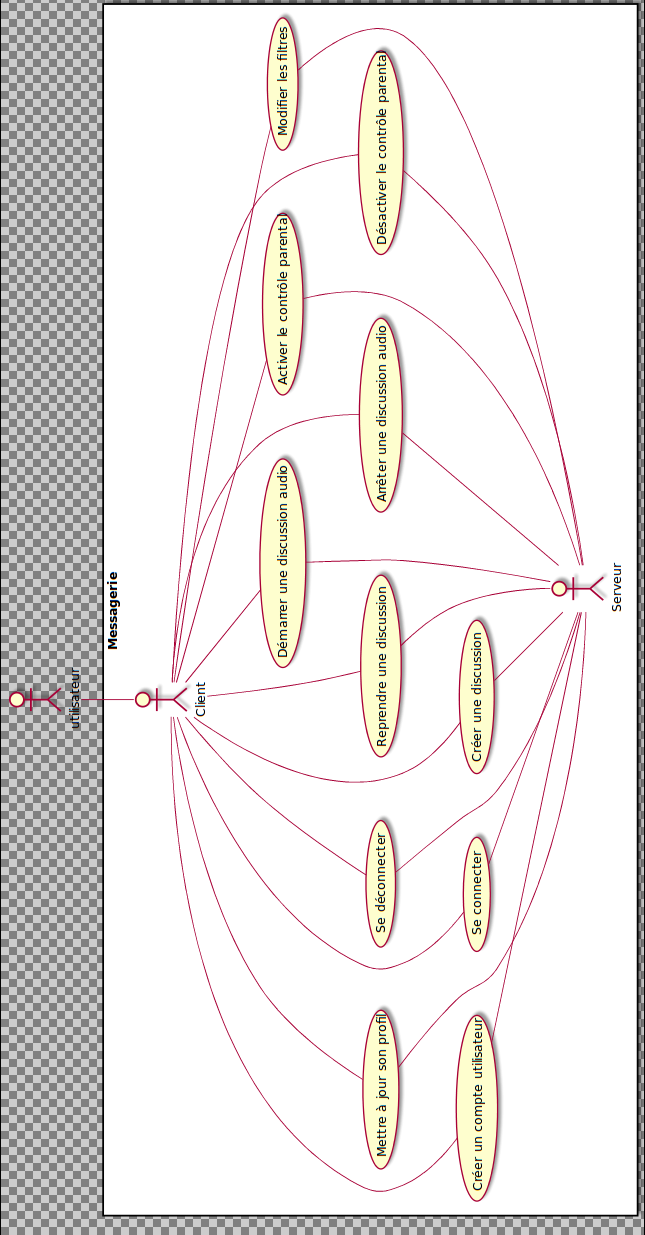
\includegraphics[scale=0.46]{img/usecase.png}
		\caption{Cas d'utilisation}
	\end{figure}
	
	
\subsection{Spécifications d’interface}

\subsubsection{Interface de l’application}

\par L’application doit être responsive design afin d’être consultable autant sur ordinateur, smartphone ou tablette, quelque soit les résolutions d’écrans. 

\par L’interface utilisateur doit être intuitive et facile d’utilisation. 

\subsubsection{Arborescence de l’application web}

\begin{itemize}
	\item Page d'accueil permettant à l’utilisateur de s'inscrire ou de se connecter à la messagerie.	
	\item Une fois connecté, la page principale de la messagerie contenant les éléments majeurs de l'application web tels que la liste des utilisateurs connectés, l’historique des dernières conversations en ligne et son espace membre avec son image de profil ou avatar.
	\item Page de discussion 
	\item Page de configuration du profil
	\item Page de configuration des filtres
\end{itemize}

\subsubsection{Maquettes}

Cette partie présentes les maquettes qui ont été réaliser avant la réalisation. 

\begin{figure}[H]
   \begin{minipage}[c]{.46\linewidth}
      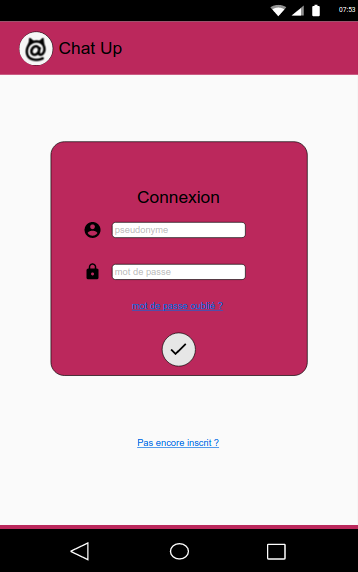
\includegraphics[scale=0.5]{img/SeConnecter.png}
      \caption{Page de connexion}
   \end{minipage} \hfill
   \begin{minipage}[c]{.46\linewidth}
      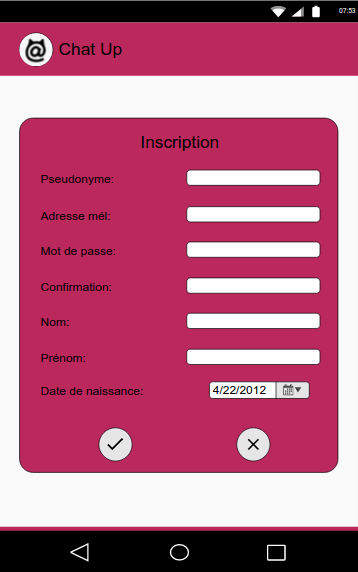
\includegraphics[scale=0.5]{img/CreerUnCompte.png}
      \caption{Page d'inscription}
   \end{minipage}
\end{figure}


\begin{figure}[H]
   \begin{minipage}[c]{.46\linewidth}
		\centering 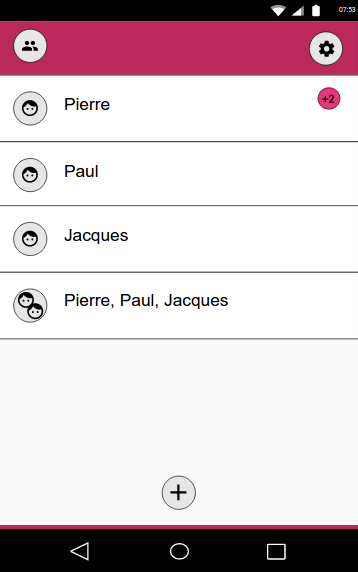
\includegraphics[scale=0.5]{img/Messagerie.png}
		\caption{Page de messagerie}
   \end{minipage} \hfill
   \begin{minipage}[c]{.46\linewidth}
		\centering 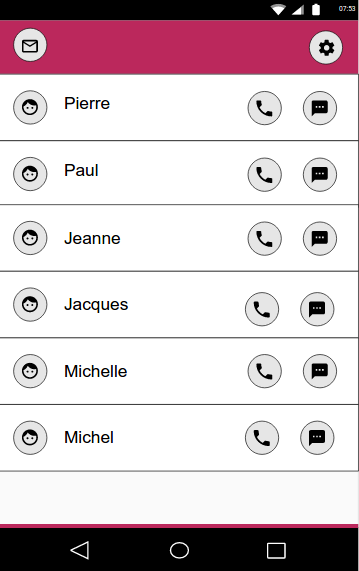
\includegraphics[scale=0.5]{img/Contacts.png}
		\caption{Page des contacts}
   \end{minipage}
\end{figure}

\begin{figure}[H]
   \begin{minipage}[c]{.46\linewidth}
		\centering 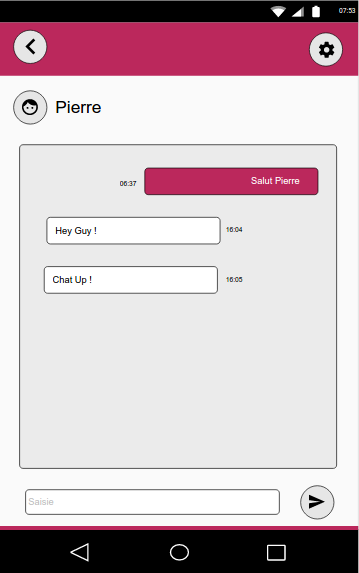
\includegraphics[scale=0.5]{img/Conversation.png}
		\caption{Conversation textuelle}
   \end{minipage} \hfill
   \begin{minipage}[c]{.46\linewidth}
		\centering 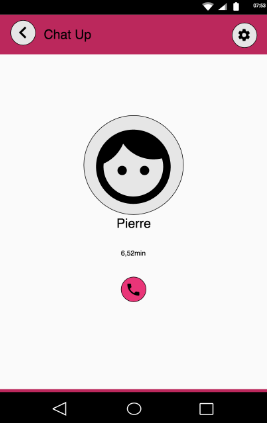
\includegraphics[scale=0.68]{img/audio.png}
		\caption{Conversation audio}
   \end{minipage}
\end{figure}


	\begin{figure}[H]
		\centering 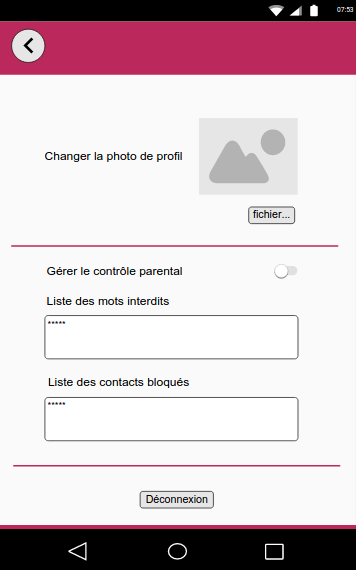
\includegraphics[scale=0.5]{img/Parametres.png}
		\caption{Page de paramètres}
	\end{figure}
	
	
\subsection{Spécifications opérationnelles}

En ce qui concerne les spécifications opérationnelles. \\

Il est préférable que l'application soit performante. La discussion doit être suffisamment rapide pour que la discussion soit instantanée. \\

En ce qui concerne la sécurité : \\

\begin{itemize}
	\item Les discussions doivent être privées et uniquement visibles par les membres de la conversation. 
	\item Les mots de passe des comptes utilisateurs ne doivent pas être stockés en clair dans la base de données.
\end{itemize}




	
\newpage
\part{Conception Préliminaire}
	\section{Conception préliminaire}

Cette partir présente la conception préliminaire qui a été réalisée.

	\subsection{Diagramme de modèle du domaine}
	Cette partie présente les diagrammes de modèle du domaine du client et du serveur.
	Le diagramme de Modèle du Domaine serveur, sur la figure \ref{diagModeleServeur}, montre la structure envisagée pour notre serveur.
	On y trouve donc une entité Serveur chargée de la communication avec le client.
	Les autres entités représentent la structure des données pour le fonctionnement de notre application.\\
	
	Les mises à jours suite à la réalisation sont apparente sur la figure.

	\begin{figure}[H]
		\centerline{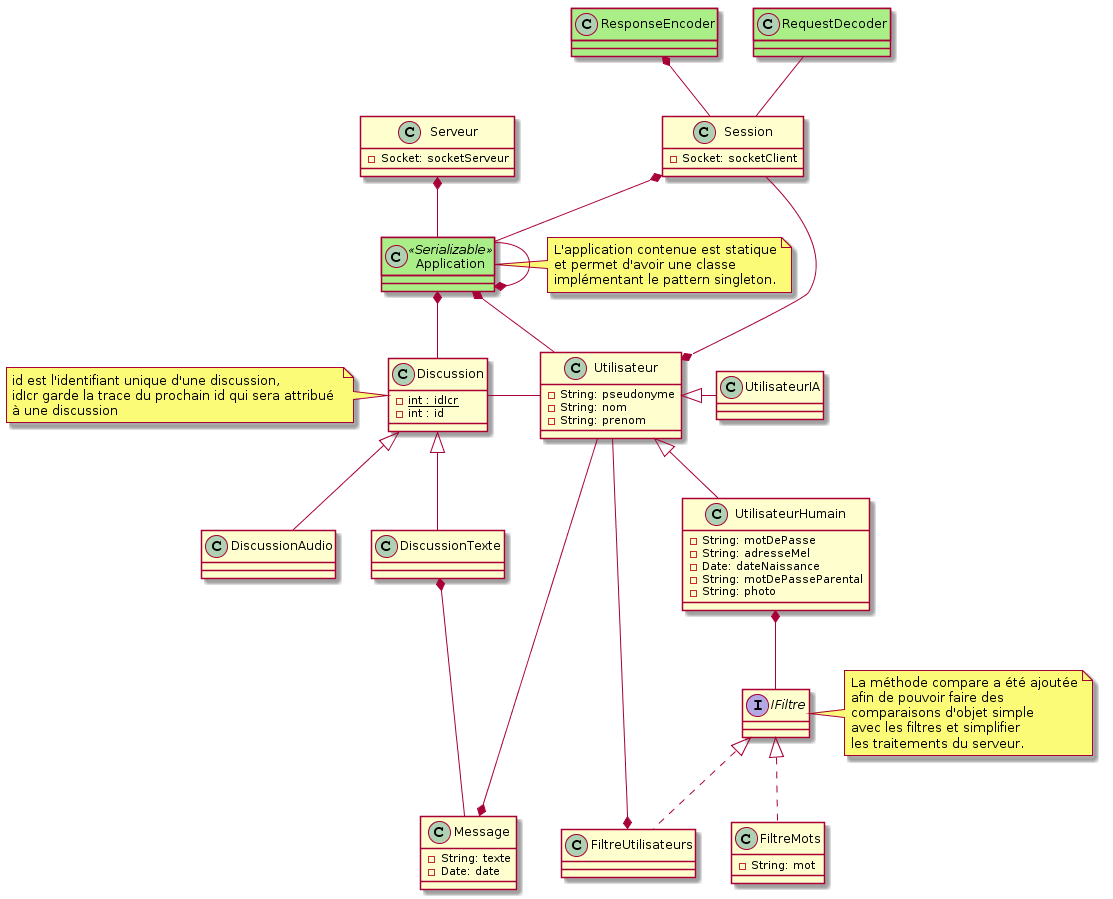
\includegraphics[width=16.5cm]{img/modeleDomaineServeurV2.png}}
		
		\caption{\label{diagModeleServeur}Diagramme de modèle du domaine côté serveur}
	\end{figure}

	\newpage

	Ce diagramme de Modèle du Domaine présente la structure générale de l'application du côté du client.
	Celui-ci réutilise la plupart des entités présentes dans le modèle du domaine du côté serveur.
	Ainsi, nous avons une cohérence entre les données des deux côtés. \\
	
		Les mises à jours suite à la réalisation sont apparente sur la figure \ref{modeleDomaineClient}.
	\begin{figure}[H]
		\centerline{\includegraphics[width=16.5cm]{img/modeleDomaineClientV2.png}}
		\caption{Diagramme de modèle du domaine côté client}
		\label{modeleDomaineClient}
	\end{figure}

	\newpage

	\subsection{Diagramme de séquence système}
	
	
	Voici un diagramme séquence système correspondant au cas d'utilisation le plus important du projet : envoyer un message
	\begin{figure}[H]
		\centerline{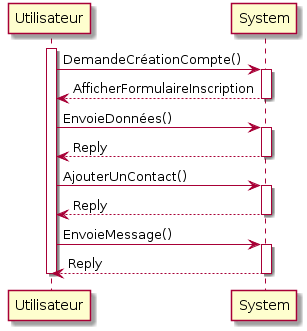
\includegraphics[width=12.5cm]{img/sequenceSystemeEnvoiMessage.png}}
		\caption{Diagramme de séquence système de l'envoi de messages}
	\end{figure}

	\newpage

	\subsection{Diagramme de navigation}
	Lorsque l'utilisateur arrive sur l'application, il arrive d'abord sur une "Page de login" où l'utilisateur a le choix entre (les champs en italique représente les modifications qui ont été effectuées) :
	\begin{itemize}
		\item connexion : entrer ses identifiants dans "Pseudonyme" et "Mot de passe" afin de se connecter en appuyant sur le bouton de validation
		\item inscription : créer un compte en cliquant sur "Pas encore inscrit ?".
		Dans ce cas, l'utilisateur arrive sur la "Page d'inscription" où il est possible d'indiquer ses identifiants "Pseudonyme", "Adresse mél", "Mot de passe", "Confirmation", "Nom", "Prénom", et "Date de naissance".
		L'utilisateur s'inscrit en appuyant sur le bouton de validation.
		L'utilisateur peut également retourner sur la "Page de connexion" en appuyant \textit{sur le bouton d'accueil}.\\
	\end{itemize}

	Lorsque l'utilisateur a passé l'étape de connexion ou d'inscription, il arrive sur la "Page de Messagerie" où il visualise les différentes conversations déjà créées. Sur cette page, différentes possibilités s'offre à lui :
	\begin{itemize}
		\item L'utilisateur peut cliquer sur une conversation déjà existante et dans ce cas il arrive sur une "Page de conversation"
		\item "Page de paramètres" : l'utilisateur peut cliquer sur l’émoticône de paramètres et dans ce cas il arrive sur la "Page de paramètres"
		\item "Page de contacts" : l'utilisateur peut cliquer sur l’émoticône des contacts, à gauche du nom de l'application, et dans ce cas il arrive sur la "Page de contacts"
		\item "Nouvelle conversation" : l'utilisateur peut cliquer sur l’émoticône "+" afin de créer une nouvelle conversation, dans ce cas une pop-up s'ouvre pour choisir un ou plusieurs utilisateurs. Il peut valider et arriver sur la "Page de conversation" associée\\
	\end{itemize}

	Lorsque l'utilisateur se situe sur une "Page de conversation", différentes possibilités s'offre à lui :
	\begin{itemize}
		\item envoyer un message en remplissant le champ et cliquer sur \textit{le bouton} envoyer
		\item "Page de paramètres" : de la même manière
		\item "Page de Messagerie" : l'utilisateur peut cliquer sur l’émoticône de \textit{Messagerie} et dans ce cas il retournera sur la "Page de Messagerie"\\
	\end{itemize}

	\newpage

	Lorsque l'utilisateur se situe sur une "Page de contacts", différentes possibilités s'offre à lui :
	\begin{itemize}
		\item appeler un contact en cliquant sur l’émoticône d'appel.
		Dans ce cas une "\textit{Page} Conversation Audio" s'ouvre, l'utilisateur pourra raccrocher en appuyant sur l’émoticône d'appel \textit{rose} afin de couper la conversation audio et retourner sur la "Page de contacts"
		\item "Page de conversation" : l'utilisateur peut cliquer sur l’émoticône de message pour contacter un contact dans une conversation privée et dans ce cas il arrive sur la "Page de Conversation" associée
		\item "Page de paramètres" : de la même manière
		\item "Page de Messagerie" : l'utilisateur peut cliquer sur l’émoticône de Messagerie, à gauche du nom de l'application, et dans ce cas il arrive sur la "Page de Messagerie"\\
	\end{itemize}

	Lorsque l'utilisateur se situe sur la "Page de paramètres", différentes possibilités s'offre à lui :
	\begin{itemize}
		\item modifier ses paramètres en remplissant les champs
		\item retourner sur la page précédente en cliquant sur l’émoticône de retour
		\item se déconnecter en cliquant sur le bouton "Déconnexion"\\
	\end{itemize}

	\begin{figure}[H]
		\centerline{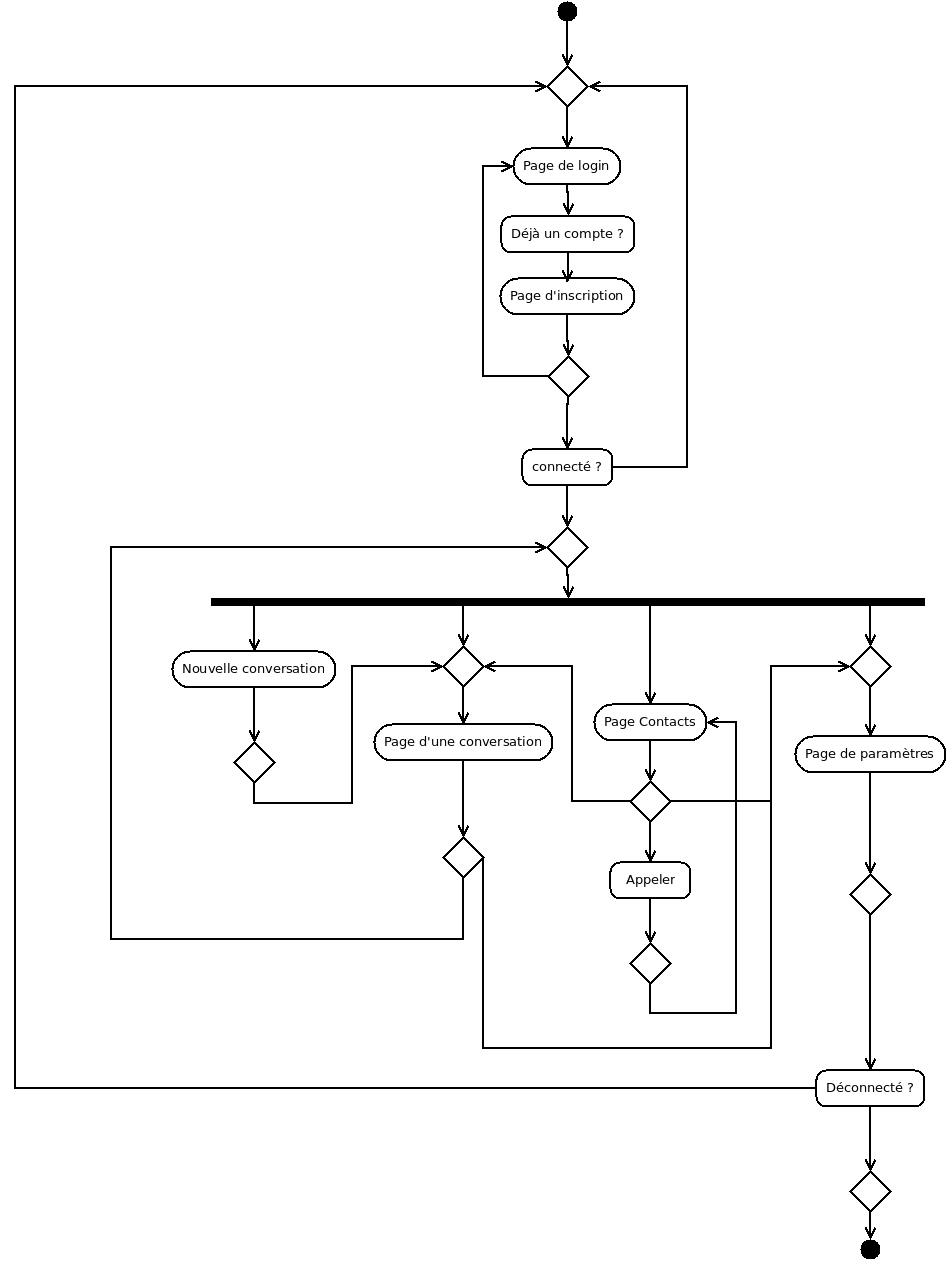
\includegraphics[width=16.5cm]{img/navigation.png}}
		\caption{Diagramme de navigation}
	\end{figure}


	\subsection{Tableau d’Interaction}
	Dans cette partie nous allons vous présenter toutes les interactions qui interviennent lors de l'envoi d'un message de la part d'un utilisateur à l'aide d'un tableau d’interaction et d'un diagramme d’interaction.

	\textbf{Tableau d’interaction pour envoyer un message :} \\

	Action de début : Vouloir envoyer un message à une personne. \\

	\begin{tabular}{|p{7cm}|p{7cm}|}
		\hline
		Action de l'utilisateur & Action du système\tabularnewline
		\hline

		\hline
		1) Entrer son login et mot de passe (A)  & \tabularnewline

		\hline
		2) Valider  & 3) Vérifier le login et le mot de passe dans la base de données\tabularnewline

		\hline
		4) Sélectionner une discussion commencée ou cliquer sur le "+" pour	démarrer une conversation avec une nouvelle personne ou aller dans les contacts et cliquer sur l’Icône message en face de la personne correspondante & \tabularnewline

		\hline
		5) Envoyer son message  & \tabularnewline
		\hline
	\end{tabular}

~\\

	Action de fin  : Message affiché dans la discussion. \\

	Exception A : Si l'utilisateur n'a pas encore de compte, la première action est de cliquer sur pas encore inscrit, ce qui envoie l'utilisateur sur la page d'inscription où il remplie le formulaire et valide.

	\begin{figure}[H]
		\centerline{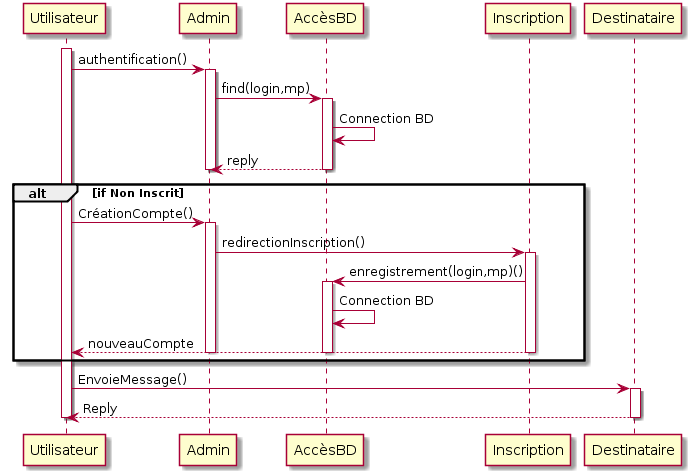
\includegraphics[width=12.5cm]{img/interaction.png}}
		\caption{Diagramme d’interaction}
	\end{figure}

	\newpage

	\subsection{Découpage en packages et les signatures externes de chaque package}
	Les deux diagrammes suivants représentent le découpage en package de notre application.
	Les packages du coté serveur et client sont idépendants même si ils utilisent des classes communes puisqu'il ne sont pas dans le même langage.
	\begin{figure}[H]
		\centerline{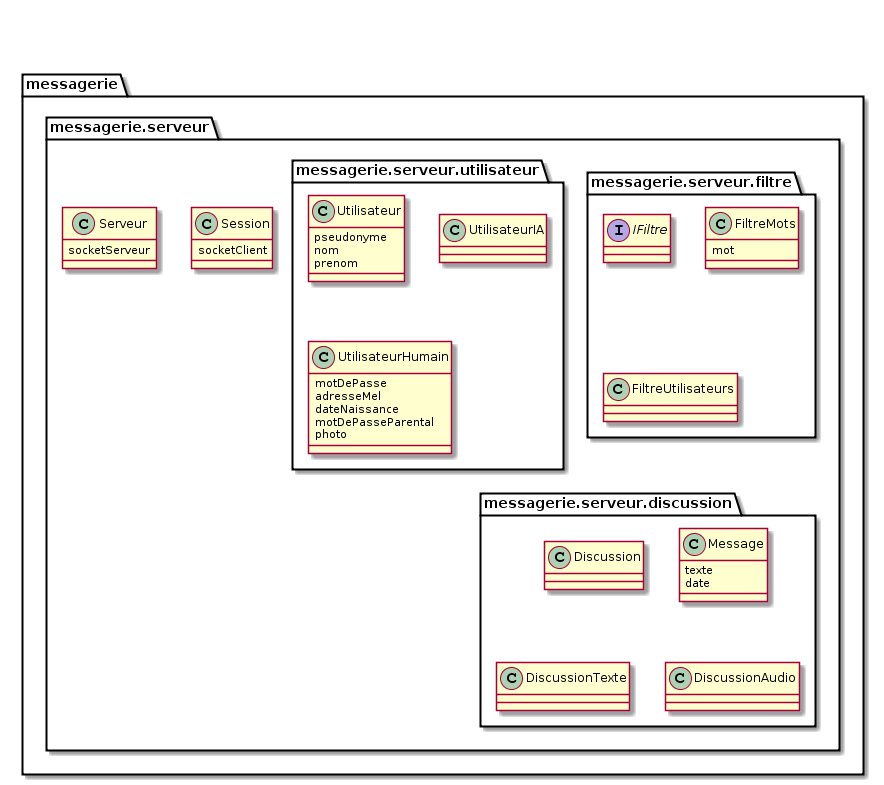
\includegraphics[width=16.5cm]{img/packageServeur.png}}
		\caption{Diagramme de package côté serveur}
	\end{figure}

	\begin{figure}[H]
		\centerline{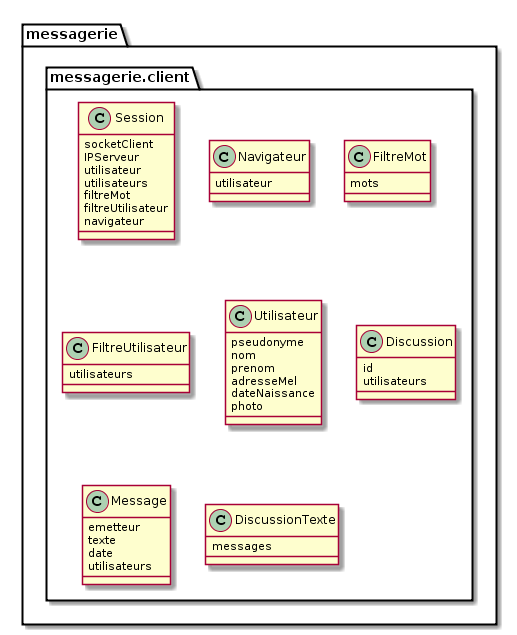
\includegraphics[width=16.5cm]{img/packageClient.png}}
		\caption{Diagramme de package côté client}
	\end{figure}
	
\newpage
\part{Perspectives}
	\section{Conception détaillée}

	\subsection{Diagrammes de classes}
	Les diagrammes de classes présentés dans cette partie se basent sur les diagrammes de modèle du domaine explicités précédemment.
	Ainsi les entités ont été reportées en classes, avec les fonctions qui leur sont associées.
	\begin{figure}[H]
		\centerline{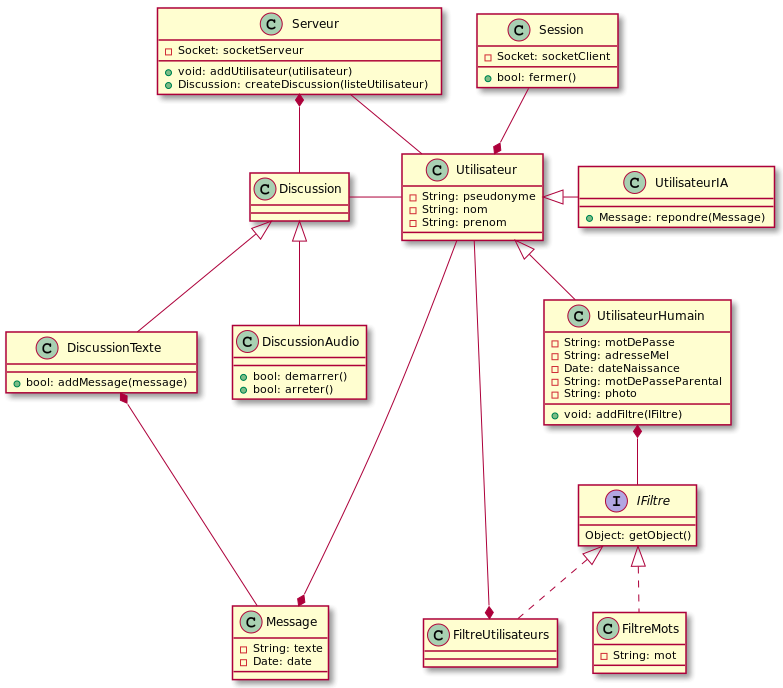
\includegraphics[width=16.5cm]{img/classesServeur.png}}
		\caption{Diagramme de classes côté serveur}
	\end{figure}

	\newpage

	Ce diagramme de classes représente la partie client de notre application, avec les attributs et méthodes des différentes classes.
	Les getter et setter ne sont pas présents sur celui-ci mais seront présents sur tout les attributs des classes Message, Discussion et Utilisateur.
	\begin{figure}[H]
		\centerline{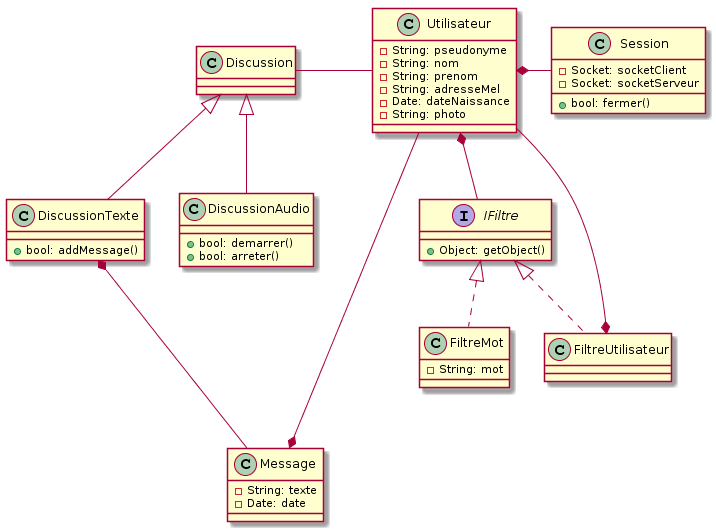
\includegraphics[width=16.5cm]{img/classesClient.png}}
		\caption{Diagramme de classes côté client}
	\end{figure}



\newpage
\part{Perspectives}
	\section{Choix technique}

\par Pour ce projet il a été décidé de réaliser l'architecture serveur/client avec un serveur en java communicant avec le client à l'aide de web socket. L’interface de la messagerie a quant à elle été réalisée à l'aide de technologies web, tout en restant dans le cadre de l'informatique réparti. 

\subsection{Le serveur}
\par Le serveur a entièrement été réalisé en java, et utilise les webSocket de la librairie java-ws pour faire la communication avec le client.
\par L'une des problématiques rencontrées lors du développement du serveur était la persistance des informations, nous avons alors exploré deux options : la sérialisation ou une base de donnée.
Au final notre choix c'est plutôt porté sur la sérialisation parce que c'est la solution simple à implémenter et convient le mieux pour un petit projet comme celui-la.
\par Les connexions reçus par le serveur sont traiter avec un système de session, chaque client a une session qui lui ai attribué lors de sa connexion, c'est la session qui permet d'envoyer et de recevoir les requêtes et réponses.
\par Les requêtes prennent forme d'objets JSON avec une action et un contenu. A la réception d'une requête la session fait appelle a un module de décodage qui décode ces requêtes en faisant un Parsing du JSON et appelle la méthode correspondante a l'action grâce a de l'introspection, le reste du contenu de la requête sera mis en paramètre de cette méthode.
\par Chaque requête déclenche l'envoi d'un objet JSON en réponse qui contient à son tour une action, un contenu et un état pour dire si le traitement c'est bien passé.

\subsection{Les web sockets}
\par Les web sockets permettent d'établir la communication entre un client et un serveur. Pour cela nous avons utilisé l'API websocket proposée par HTML pour le client 
et l'API websocket de Java pour le serveur, ce qui nous permet de faire de la communication en temps réel.

\par Les websocket sont une surcouche aux sockets intégrant au dessus un protocole en différentes étapes.
Tout d'abord, au moment de la connexion, le client et le serveur doivent effectuer ce que l'on appelle une poignée de main.
Cette étape permet d'assurer qu'ils sont capables de communiquer sans problème et de définir les modalités d'envoi de message.
Après cette étape, la communication est établit entre le client et le serveur et ils peuvent décider de communiquer l'un avec l'autre 
quand ils le souhaitent sans contrainte de temps, la connexion mise en place étant permanente. 
L'envoi des messages est masqué à l'aide d'un cryptage XOR que le destinataire est capable de décoder.

\section{Guide d'utilisation}

\par Pour lancer l'application il est nécessaire de lancer le serveur puis le client. Pour lancer le serveur il suffit de lancer le compile.sh et le run.sh du dossier serveur et pour lancer le client il faut lancer la commande gulp puis la commande node express.js qui permet d'accéder à la page de connexion sur le navigateur. \\


\par Cette application de messagerie se compose de la manière suivante : \\

\par Au début l'utilisateur accède à une page de login qui lui permet de renseigner son pseudonyme et son mot de passe afin d'accéder au service de messagerie. Si l'utilisateur est nouveau, il a la possibilité de créer son compte en renseignant son pseudonyme, adresse mél, mot de passe, nom, prénom et date de naissance. 
\par Une fois l'authentification faite l'utilisateur accède à la page principale qui correspond à la page d'historique des conversations des utilisateurs. L'utilisateur peut ainsi sélectionner une conversation déjà existante ou bien en créer une nouvelle. Il a la possibilité de choisir parmi les membres du service messagerie la personne qu'il veut joindre. Il accède ensuite à la page de cette nouvelle conversation. Il peut discuter avec les personnes membres de la messagerie ou bien avec l'IA : MiaBot.
\par Via la navbar il est possible d'accéder au carnet d'adresse et à la page de paramètres. \\

Voici les captures d'écran de l'application que nous avons réalisée.



\begin{figure}[H]
   \begin{minipage}[c]{.46\linewidth}
      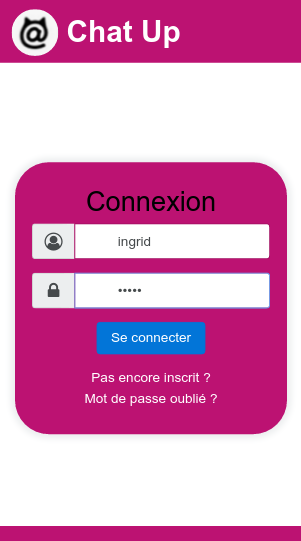
\includegraphics[scale=0.5]{img/01Login.png}
      \caption{Page de connexion}
   \end{minipage} \hfill
   \begin{minipage}[c]{.46\linewidth}
      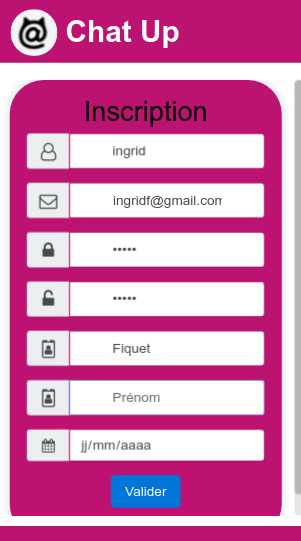
\includegraphics[scale=0.5]{img/02InscriptionChamp.png}
      \caption{Page d'inscription}
   \end{minipage}
\end{figure}


\begin{figure}[H]
   \begin{minipage}[c]{.46\linewidth}
		\centering 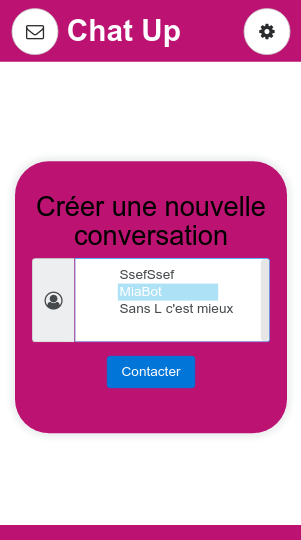
\includegraphics[scale=0.5]{img/03ChoixMsg.png}
		\caption{Page de Création d'une conversation}
   \end{minipage} \hfill
   \begin{minipage}[c]{.46\linewidth}
		\centering 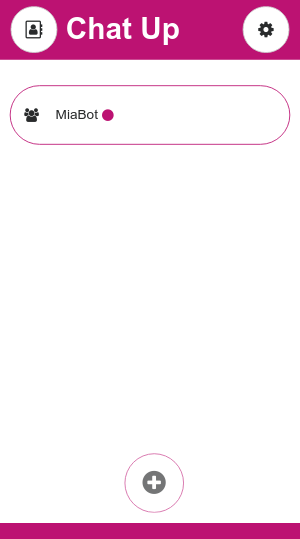
\includegraphics[scale=0.5]{img/05HistoriqueMessagerie.png}
		\caption{Page de Messagerie}
   \end{minipage}
\end{figure}

\begin{figure}[H]
   \begin{minipage}[c]{.46\linewidth}
		\centering 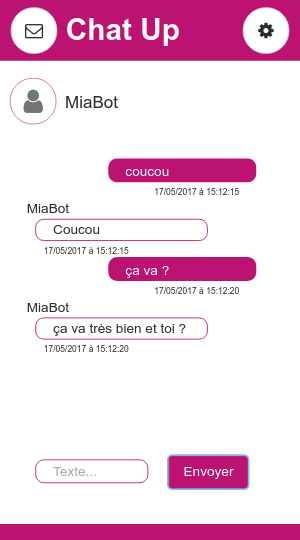
\includegraphics[scale=0.5]{img/04Messagerie.png}
		\caption{Conversation textuelle}
   \end{minipage} \hfill
   \begin{minipage}[c]{.46\linewidth}
		\centering 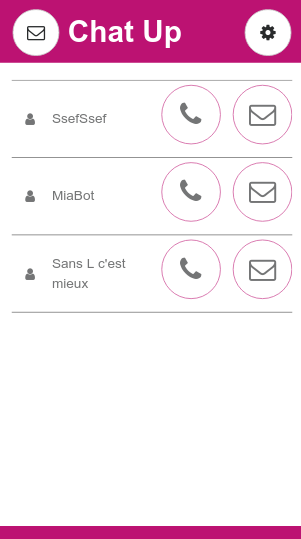
\includegraphics[scale=0.5]{img/06ContactMessagerie.png}
		\caption{Page de contacts}
   \end{minipage}
\end{figure}


\begin{figure}[H]
   \begin{minipage}[c]{.46\linewidth}
		\centering 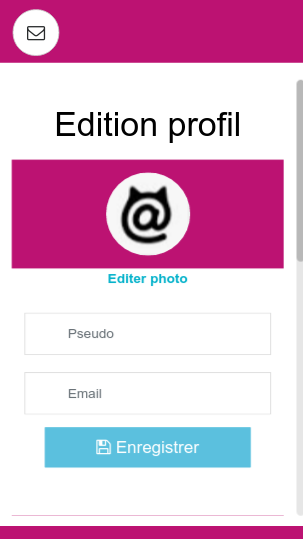
\includegraphics[scale=0.5]{img/07Param.png}
		\caption{Page de paramètres}
   \end{minipage} \hfill
   \begin{minipage}[c]{.46\linewidth}
		\centering 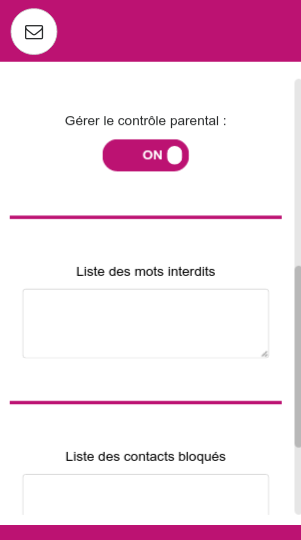
\includegraphics[scale=0.5]{img/08paramsuite.png}
		\caption{Page de paramètres}
   \end{minipage}
\end{figure}

 


\section{Tests de validation}

Voici la liste des tests de validation qui ont été réalisés. \\

%TODO mettre que les tests qui ont été réalisé 

\paragraph{Spécifications fonctionnelles\\} 

Voici la liste des tests qui ont été réalisés techniquement :
\begin{itemize}
	\item Créer un nouveau compte ;
	\item Obtenir la liste des conversations ;
	\item Créer une conversation ;
	\item Faire une conversation avec plusieurs utilisateurs dans une conversation textuelle ; 
	\item Créer des filtres (du côté serveur);
\end{itemize}

Les tests suivant ont été réalisés de manière manuelle : 
\begin{itemize}
	\item Se connecter et se déconnecter ;
	\item Voir la liste des autres utilisateurs ;
	\item Envoyer un message dans une conversation ;
	\item Recevoir un message dans une conversation ;
	\item Voir l'historique d'une conversation après reprise ;
	\item Activer et désactiver le contrôle parental ;
	\item Créer des filtres (du côté client);
	\item Filtrer des messages ; 
	\item Avoir une conversation minimaliste avec l'IA ; \\
\end{itemize}

\paragraph{Spécifications d'interface \\}

En ce qui concerne les spécifications d'interface, nous avons bien réalisé une application responsive design, consultable sur un écran de taille d'ordinateur, de tablette ou de smartphone. De plus, l'application est intuitive et facile d'utilisation.

\paragraph{Spécifications opérationnelles \\}

Nous avons répondu aux spécifications opérationnelles suivantes :
\begin{itemize}
	\item Rapidité de la discussion instantanée ; 
	\item Discussions privées et uniquement visibles par les membres de la conversation ;
	\item Mot de passe hashé. \\
\end{itemize}
	
\newpage
\part{Conclusion}
	
Parmi les fonctionnalités que nous n'avons pas réalisé figurent : 

\begin{itemize}
	\item Discussion audio ;
	\item Indiquer si l'utilisateur est connecté ou hors ligne ;
	\item Avatar 3D lors de la conversation audio ;
	\item Affichage d’emojis ;
\end{itemize}

\par Cela s'explique principalement par le fait que nous avons manqué de temps pour la réalisation des discussions audio qui aurait nécessité beaucoup de temps.

\par De même pour la mise en place d'avatar animé et de l'affichage d'emoji dans les conversations qui n'étaient pas des fonctionnalités primordiales.  \\


\par En ce qui concerne l’amélioration de notre projet nous pouvons suggérer une amélioration du point de vu de l'IA.

\par En effet, la version actuelle de l'IA est très minimaliste. Elle fonctionne avec une reconnaissance de la question de l'utilisateur au mot près afin d'y associer une réponse. Pour cela le programme de l'IA définit des catégories de questions de l'utilisateur et de réponses de l'IA par thématique. Ces catégories sont chacune décris par un fichier xml qui contient toutes les réponses de l'IA possibles selon la thématique et toutes les questions possibles de l’utilisateur selon la catégorie. Ainsi quand l'utilisateur pose une question, le programme reconnaît la catégorie de la conversation et choisit une réponse de façon aléatoire dans le fichier de réponses correspondant à la bonne catégorie de l'IA. 

\par Cette solution n'est donc pas efficace pour une vraie conversation car il faut prévoir à chaque fois tous les cas possibles. Actuellement diverses solutions permettent d'intégrer des chatbots à des sites web en définissant à travers une API, ou un langage (par exemple AIML) toutes les règles de fonctionnement de l'IA. Ainsi les plate-formes qui proposent ces services mettent à disposition des algorithmes très puissants de réseau de neurones notamment qui permettent de simuler une conversation humaine. Parmi les solutions actuelles on peut citer l'API de Google : API.AI qui permet de développer, entraîner et déployer son propre chatbot. 

\par Une autre amélioration serait de mettre en place un base de donnée pour sauvegarder les données. La sérialisation mise en place actuellement a quelques défauts notamment l'impossibilité de lire la sauvegarde après n'importe quelle modification du code.

\par Un dernier point d’amélioration serait d’améliorer la gestion des erreurs entre le client et le serveur, actuellement le serveur envoie un simple attribut boolean qui prend la valeur faux sans avoir plus d'information sur l'erreur. Ce qui serais intéressant, c'est de mettre des codes d'erreurs pour les différents types d'erreur (comme pour le protocole http) et la possibilité d'ajouter un message d'erreur.

\newpage
\part{Conclusion}

\par Parmi les fonctionnalités principales prévues nous avons réalisé toutes les fonctionnalités basiques et implémentés des fonctionnalités supplémentaires. \\

\par Ainsi, l'utilisateur peut créer un compte sur l'application, se connecter et se déconnecter. L'utilisateur a la possibilité de créer une conversation avec un ou plusieurs utilisateurs. 
\par Lors d'une conversation à plusieurs, alors tous les utilisateurs reçoivent les messages des autres utilisateurs instantanément. Après avoir créé ses conversations, alors l'utilisateur peut avoir accès à la liste des ses conversations existantes.
\par Lorsque l'utilisateur retourne sur une conversation déjà existante, alors l'historique de cette conversation apparaît.
\par Un système de contrôle parental a été mis en place avec la possibilité de filtrer certains mots. Il suffit de rentrer les mots à filtrer séparés par des espaces, dans le système de filtre présent dans les paramètres. Ainsi lorsque le mot sera envoyé par un contact, alors ce mot sera remplacé par des étoiles.
\par Enfin nous avons mis en place \\


	%TODO Image de profil pour chaque utilisateur. ??

En ce qui concerne, les fonctionnalités qui auraient pu être ajoutées mais qui n’ont même pas été prévues dans les spécifications, après les discussions discussion audio, il serait parfait d'ajouter une fonctionnalité de vidéo et de visio conférence. 

\newpage
\part{Annexe}

\end{document}
